% !TeX document-id = {759b9040-8a7f-4d09-8f16-a89e0a780c65}
%%% Magic comments for setting the correct parameters in compatible IDEs
% !TeX encoding = utf8
% !TeX program = pdflatex 
% !TeX spellcheck = en_US
% !BIB program = biber



\documentclass[notitlepage,english]{hgbreport}
\usepackage{listings}
\usepackage[utf8]{inputenc}
\usepackage{cleveref}



%acronyms
\newcommand{\Acronym}[1]{{#1}}
\newcommand{\LBP}{\Acronym{LBP}}
\newcommand{\SFM}{\Acronym{SFM}}

%-----
\newcommand{\Vertices}{\mathcal{V}}
\newcommand{\Edges}{\mathcal{N}}
\newcommand{\Graph}{\mathcal{G}}

%---------------------------------------------

\graphicspath{{images/}}  % where the images at?
\bibliography{references}  % requires file 'references.bib'

%%%----------------------------------------------------------
\author{Giorgio Mariani}										% your name
\title{IM490 Depth-Map Recovery from RGB-video\\	% the name of the course or project
				\textbf{Project 1 Report}}	% or "Project Report"
\date{\today}
%%%----------------------------------------------------------


%%%----------------------------------------------------------
\begin{document}
%%%----------------------------------------------------------

\maketitle

\begin{abstract}\noindent
%This document is a simple template for a typical term or semester paper (lab/course report, ``Übungsbericht'', \etc) based on the \textsf{HagenbergThesis}\footnote{See \url{https://github.com/Digital-Media/HagenbergThesis} for the most current version
%and additional examples.
%This repository also provides a good introduction and useful hints for authoring academic texts with LaTeX.}
%The structure and chapter titles have been formulated to provide a good starting point for a typical \emph{project report}.
%This document uses the custom class \textsf{hgbreport} which is based on \latex's standard \textsf{report} 
%document class with \texttt{chapter} as the top structuring element. 
%If you wish to write this report in German you should substitute the line
\bigskip
\noindent
%Use the abstract to provide a short summary of the contents in the document.
\end{abstract}


%%%----------------------------------------------------------
\tableofcontents
%%%----------------------------------------------------------



%%%----------------------------------------------------------
\chapter{Aims and Context}
%%%----------------------------------------------------------

%Describe the initial goals and situation that lead to this project, requirements, as well as references to related work (\eg, \cite{Higham1998}).




\section{Introduction}
\label{sec:introduction}
% describe problem

The aim of this project is the implementation of the article \textit{"Consistent Depth Map Recovery from a Video Sequence"} \cite{Zhang2009}, by Zhang, Jia, Wong, and Bao and published in \textit{Transaction on Pattern Analysis and Machine Intelligence} (TPAMI).
%The article describes an algorithm which is able to generate a sequence of \emph{depth-maps} starting from an RGB-video.
The problem faced by Zhang et al. consists in the estimation of a sequence of \emph{depth-maps}\footnote{A \emph{depth-map} is an image in which each pixel maintains depth information.} starting from an RGB-video.
More precisely, given an image sequence representing a video of a static scene, the aim of the paper is to estimate a sequence of images with consistent depth values for each pixel and frame.
This depth values can then be  used for a variety of tasks, such as scene reconstruction and layer separation.
\begin{figure}[!h]
	\centering
	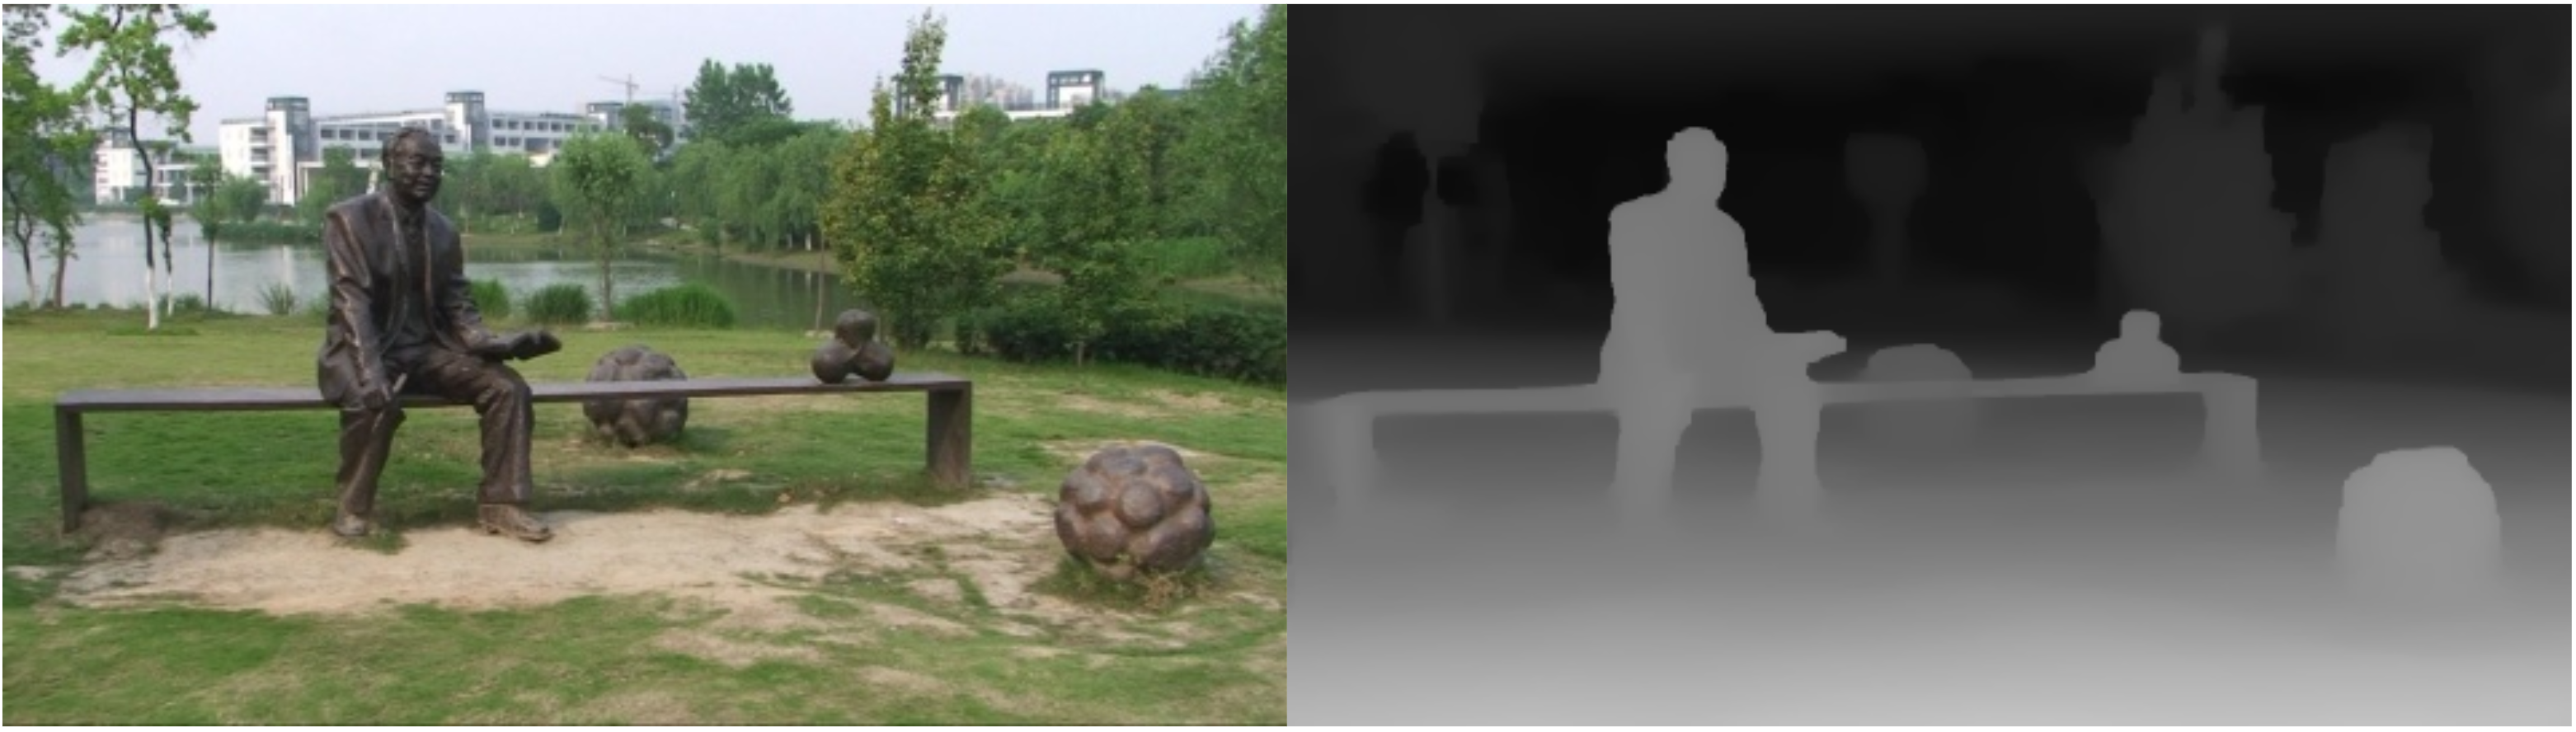
\includegraphics[width=.95\textwidth]{depthmap_example.png} %{CS0031}
	\caption{One of the estimated depth-map  obtained using \cite{Zhang2009} over a sequence of 200 images.}
	%\label{fig:CocaCola}
\end{figure}

While a free implementation is available on the authors' website~\cite{CVGweb}, they do not offer its source code; hence, the reasons behind this project are to offer an open-source implementation of said article, and to offer didactic improvement for the project's author.

\section{Proposed Approach}
% overview of proposed solution
The approach proposed in the original article consists of four steps:
\begin{enumerate}
	\item Camera Parameter Estimation
	\item Depth-maps Initialization
	\item Depth-maps Bundle Optimization
	\item Depth-maps Space-Time Fusion
\end{enumerate}

\paragraph{Camera parameter estimation:} During this phase, the camera parameters (\ie \emph{position}, \emph{rotation}, and \emph{intrinsic matrix}) are estimated, using a \emph{Structure From Motion} (STM) algorithm; unsurprisingly, the one used in the article is the same as the one described in \cite{Zhang2007}, with Zhang and Bao two of the article's authors.

\paragraph{Depth-maps initialization:} 
For each frame in the video a raw estimation of the corresponding depth-map is computed; this is achieved by minimizing a (per-frame) energy function whose parameters are the depth values to estimate.

These raw depth-maps are successively processed using a plane fitting algorithm; each image is divided into segments using \emph{mean-shift color segmentation} \cite{Comaniciu202}. Each segment is then considered as a plane and fitted to the existing depth-maps raw values. The resulting images are the initialized depth-maps, ready to be used in the next step.

\paragraph{Depth-maps bundle optimization:} The depth-maps obtained during the initialization process are then refined by applying geometric constraints. This refinement process iteratively elaborates the given raw data by minimizing an energy function similar to the one used in the previous step, but enriched with geometric constraints over the initialized depth-maps values (that is, the depth values between frames should be consistent).

\paragraph{Depth-maps space-time fusion:} This is the final step of the process, and it is used to polish the results obtained from the previous steps and removing eventual remaining noise.

The estimated depth-map values are used to define a loss function  that can subsequently be optimized through the use of \emph{Coniugate Gradient Method}, an optimization technique similar to \emph{ Gradient Descent}.
The designed loss function takes into consideration \emph{spatial continuity} between already computed depth-values, as well as temporal coherence and the sparse points that can be obtained by the SFM algorithm  used to compute the camera parameters.

 

\section{Related Work}
Since the proposed approach makes use of a variety of techniques, and it is relatively old (2009), the related work section is organized as follows:
\begin{enumerate}
	\item Previous work related to individual algorithms used in the proposed method.
	\item Work that makes use or improves the proposed solution. 
	\item More recent work that uses a neural network approach.
\end{enumerate}
\subsection{Previous Work}
%[TODO]
\subsection{Future Work}
%[TODO]
\subsection{Neural Network Approaches}
%[TODO]
%CNN approaches




%%%----------------------------------------------------------
\chapter{Project Details}
%%%----------------------------------------------------------
%Describe important project steps, \eg, the rationale of the chosen architecture or technology stack, design decisions, algorithms used, interesting challenges faced on the way, lessons learned \etc


\section{The Architecture}
The systems is written using the \emph{Python Programming Language}; the reason behind this decision is the relative good performance that vectorized computation libraries can achieve on python, the flexibility and simplicity of the language, and the author's past experience with python libraries such as \emph{NumPy} and \textbf{TensorFlow} makes the development less laborious.
%TODO say python version

\subsection{Dependencies and Third Party Libraries}
\paragraph{NumPy:} The main library used for computations in the project is the \textbf{NumPy} module: it is set of function designed for intensive computing in vectorized fashion, similarly to the \textbf{MATLAB} programming language.

\paragraph{OpenCV:}
The \textbf{OpenCV} library (version 4.0.0) is also utilized in the project, using the official python bindings.
\textbf{OpenCV} offers real-time computer vision by exploiting (whenever possible) accelerated hardware, such as GPUs.
Unfortunately, the official bindings are available only for python 2.7.\textit{x} interpreter, forcing the author to use a compatible interpreter.
% TODO explain why OpenCV was chosen

%\subsection{Problems Encountered with OpenCV}



\section{Approach in Detail}
% in this section I will explain the implementation of each algorithm more in detail
 
\subsection{Initialization Phase}
During the initialization phase, an initial depth-map is estimated for each frame in the input video; this estimation occurs in a two steps process: firstly, the depth-maps are initialized using Loopy Belief Propagation (\LBP) \cite{Felzenszwalb2006}, thereafter,  \emph{mean-shift segmentation} and plain fitting are used to refined the obtained results.

The video's image sequence is denoted by the sequence $I_0, I_1 ... I_m$, with $I_t$ representing the image at time $t$. The camera parameters are denoted with $K$, $R$, and $T$, which are respectively \emph{intrinsic matrix}, \emph{Rotation}, and \emph{Position}.


\paragraph{}
\LBP{} is a dynamic programming algorithm that can be used to find good approximations for energy minimization problems defined over labeled graphs (see \cref{app:LBP} for more information).




The \LBP{} algorithm requires the following inputs: a graph with vertices $\Vertices$ and edges $\Edges$, a set $D$ of possible vertex labels, a function $V$ that maps label pairs to real values and an array $U_x$ (for each vertex $x$) mapping labels to real values. The algorithms then  finds an label assignment $d_x$, for each vertex $x$ in the graph, such that the energy function \ref{eq:lbp-example-energy} is locally minimized.

Suppose to want to estimate the depth-map for an image $I$ in the sequence $I_0 ... I_m$, using \LBP; in such case, the graph nodes (the set $\Vertices$) are the image's pixels, furthermore, each node has as neighborhood the (at most) four adjacent pixels.
The labels (set $D$) represents the depth values that should be estimated. 
the edge function $V$ can be defined as
$$
V(d_x, d_y) = \lambda(x,y)\cdot\min\{|d_x - d_y|, \eta\}
$$
with $\eta$ a constant value and $\lambda$ a smoothness weight proportional to the disparity in color of an edge (\ie{} the more the $I(x)$ is distant from $I(y)$ the smaller $\lambda(x,y)$ is).
This definition for $V$ entice the difference between adjacent to not be more smooth, especially if said adjacent vertices are similar in color, and it is compliant with the \LBP{} requirements\footnote{Only a specific class of edge functions can be used for \LBP.}.

Finally, each $U_x(d)$ value is computed by projecting the pixel position  for a particular time instant $t$, using the depth-label $d$ and the camera parameters. The difference between the original pixel position color and the projected position color at time $t$ is then used to describe the likeness that $d$ is an acceptable depth-value for the pixel $x$. Summing and normalizing these differences for all time instants $t$ gives the actual value $U_x(d)$.
{
	\newcommand{\Projected}{\overrightarrow x^t(d)}
\begin{align}
	L_x(d) &= \sum_{t} \frac{\sigma_c}{\sigma_c + ||I(x) - I_t(\Projected)||}\\
	U_x(d) &= 1 - u(x) \cdot L_x(d)
\end{align}
where $\sigma_c$ is a constant value, $\Projected$ is the projection of pixel $x$ using the camera parameter at time $t$ and depth $d$, and $u(x)$ is a normalization factor such that 
$$\max_{d\in D} \{u(x)\cdot L_x(d)\} = 1$$
}

\subsection{Bundle Optimization Phase}
[TODO]
\subsection{Space-Time Fusion}
[TODO]


\section{Lessons Learned}
% express the learned lessons (how I should have been more organized with the project, and how it is not a good idea to choose an architecture have little to none experience with it ,also consider the fact that understanding the paper was not difficult even with little CV background)




%%%----------------------------------------------------------     
\chapter{System Documentation}
%%%----------------------------------------------------------
%Give a well-structured description of the architecture and the technical design of your implementation, with sufficient granularity to enable an external person to continue working on the project.
\newcommand{\ComputeEnergy}{\texttt{compute\_energy}}
\newcommand{\Estimate}{\texttt{estimate}}
\newcommand{\Lbp}{\texttt{lbp}}
\newcommand{\Utils}{\texttt{utils}}
\newcommand{\Params}{\texttt{params}}

\section{Dependencies Installation}
%show how to install opencv and various requirements

\section{Running the System}
%In order to estimate the depth-map of a 
The system can be executed by executing the following command from the operating system's command line terminal:
\begin{lstlisting}[stepnumber=0]
	python estimate.py [-i][-b] <config.txt>
\end{lstlisting}
with \texttt{<config.txt>} a configuration file containing parameter values and paths to the folder storing the data necessary for the estimation process (\ie{} either pictures or depth-maps).
The options \texttt{-i} and \texttt{-b} are used to communicate the system which steps should be executed:
%TODO explain the options

\subsection{Special Folders and Files}
Different folders and files are used by the system during depth estimation; these are divided into three types: \emph{configuration files}, \emph{picture-folders}, and finally \emph{depth-folders}.

\paragraph{Configuration File.} The configuration file is used to set the parameter values to be used while running the system, it contains key-value pairs (with syntax \texttt{<\emph{key}>=<\emph{value}>}).
Each of these pairs must be interleaved by a newline character to the next one.

These pairs specify the parameters values used in the various algorithms, as well as more practical information, like the directories storing the input image sequence or the output depth-maps. Generally speaking, this file contains all the information necessary for the system in order to work properly. Most of these parameters have default values,so they are not required to be present in the configuration file, that is, with the exception of the first few lines: indeed, the first three lines in the file must set the values for the keys \texttt{picture\_folder}, \texttt{depth\_folder\_input} (whose value is not used if the initialization step is being executed), and \texttt{depth\_folder\_output}, which will contain the estimated depth-maps.

%TODO add brief explenation of common parameters, add all parameters in appendix


\section{Python Modules}
A variety of custom modules were created for the project, an exhaustive list is the following:
\begin{description}
	\item[\ComputeEnergy:] This module contains all functions necessary for the energy computation of a single frame.
	\item[\Estimate:] This module is used to estimate the depth-maps for a sequence of images. To do so, it makes use of the module \textbf{compute\_energy}.
	\item[\Lbp:] It contains an implementation of the \emph{Loopy Belief Propagation} algorithm.
	\item[\Utils:] This module contains a variety of class that are used by the other python modules, as well as debugging and visualization procedures.
	\item[\Params:] It contains parameters to be used by the system and the various algorithms.
\end{description}
\subsection{\ComputeEnergy}
\subsection{\Estimate}
\subsection{\Lbp}
\subsection{\Utils}
\subsection{\Params}






%%%----------------------------------------------------------
\chapter{Summary}
%%%----------------------------------------------------------

%Give a concise (and honest) summary of what has been accomplished and what not. 
%Point out issues that may warrant further investigation.


\appendix %%%-----------------------------------------------


%%%----------------------------------------------------------
\chapter{Supplementary Materials}
%%%----------------------------------------------------------

%The appendix is a good place to attach a user guide, screenshots, installation instructions etc.
%Add a separate chapter for each major item.

\section{Loopy Belief Propagation Algorithm}
\label{app:LBP}
\emph{Loopy Belief Propagation} (\LBP) \cite{Felzenszwalb2006} is a dynamic programming algorithm, which can be used to calculate approximate solution for energy minimization problems defined over labeled graphs. 

\LBP{} is a specialization of the Belief Propagation (\Acronym{BP}) algorithm used for \emph{marginal distribution} approximation of \emph{Markov Random Fields}. \LBP{} is able to achieve better performance than regular \Acronym{BP} by making assumptions on the structure of the input graph and energy function.
Inputs of the \LBP{} algorithm are:
\begin{itemize}
	\item A grid graph $\Graph$ with vertices $\Vertices$ and edges $\Edges$. This graph is usually used to represent an image; each node is a pixel, and each vertex is connected to the (at  most four) adjacent pixels. 
	\item An arbitrary finite set of labels $D$. This label set is usually $\{0, ... , n\}$.
	\item A function $V$ that associates pairs of labels to values in $\R$.
	\item Two-dimensional table $U$ that associates nodes and labels to values in $\R$. The notation $U_x(d) = \alpha$ with $x\in\Vertices$, $d\in D$, and $\alpha \in \R$ is used to indicate table elements.
\end{itemize}
The algorithm can then be used to compute a mapping (denoted as $d_x$) from vertices to labels, such that the following energy function is locally minimized:
\begin{equation} \label{eq:lbp-example-energy}
E(D) = \sum_{(x,y)\in \Edges} V(d_x,d_y) + \sum_{x\in\Vertices} U_x(d_x) 
\end{equation}


%%%----------------------------------------------------------
\MakeBibliography[nosplit]
%%%----------------------------------------------------------


\end{document}
